\chapter{Implementation}

This section describes the implementation of social network site
and how the system scales.

The system is composed by the following components: (1) The Social Networking engine, which runs all PHP scripts and described in section \ref{sec:implementaion_of_social_netowrk} (2) the Social Network MySQL database, (3) The CDO server - client components and the CDO repository, and (4) the Memcached caching system, which described in section \ref{sec:memcache_implementation}.
The overall architecture of Social Network is shown at figure\ref{fig:system_architecture}

\begin{figure}[h]
	\caption{The overall architecture of Social Network.}
	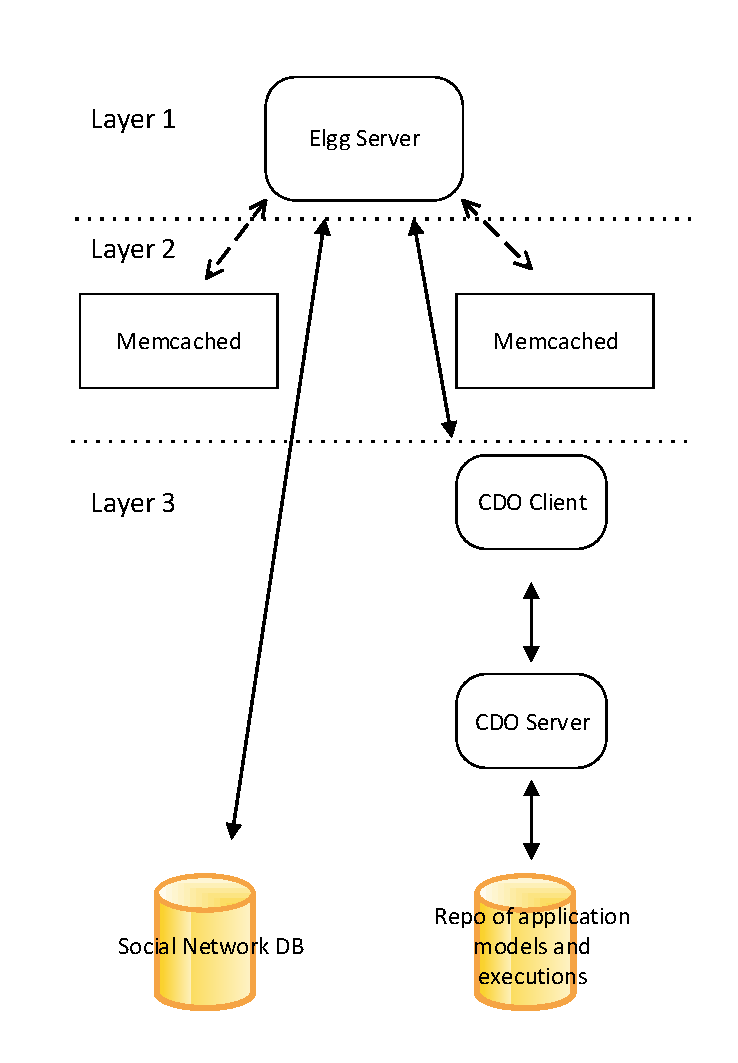
\includegraphics[width=0.6\textwidth,natwidth=200,natheight=150]{./fig/system_architecture.pdf}
	\centering
	\label{fig:elgg_architecture}
\end{figure}

Achieving the scalability of the system, two system architectures are examined at the two layers of the system. We added more than one Social Network engine in the first layer of the system. In order to keep the file system in consistent mode we integraded Apache Zookeeper\cite{zookeeper_url}.

\section{Implementation of Social Network}
\label{sec:implementaion_of_social_netowrk}
The social networking platform is implemented over the extensible Elgg social network framework\cite{elgg_url}.  Elgg is open source software written in PHP, uses MySQL for data persistence and supports jQuery~\cite{jquery_url} for client-side scripting.  The Elgg framework is structured around the following key concepts:
\begin{itemize}
\item \emph{Entities}, classes capturing social networking concepts: users, communities, application models, etc.
\item \emph{Metadata} describing and extending entities (e.g., a response to a question, a review of an application model, etc.).
\item  \emph{Relationships} connecting two entities (e.g., user A is a friend of user B, user C is a contributor to an application model, etc.).
\end{itemize}
All Elgg objects inherit from ElggEntity, which provides the general attributes of an object. Elgg core comes with the following basic entities: ElggObject, ElggUser, ElggGroup, ElggSite, ElggSession, ElggCache, as well as other classes necessary for the operation of the engine.

Elgg comprises a core system that can be extended through plugins (examples are the Cart system or the handling of Application Models). Plugins add new functionality, can customize aspects of the Elgg engine, or change the representation of pages.
A plugin can create new objects (e.g., ApplicationObject) characterized (through inheritance of ElggEntity) by a numeric globally unique identifier (GUID), owner GUID, Access ID. Access ID encodes permissions ensuring that when a page requests data it does not touch data the current user does not have permissions on. 

Figure\ref{fig:elgg_architecture} shows the model, view, and control parts of Elgg's architecture. In a typical scenario, a web client requests an HTML page (e.g., the description of an application model).  The request arrives at the \emph{Controller}, which confirms that the application exists and instructs \emph{Model} to increase the view counter on the application model object. The controller dispatches the request to the appropriate handler (e.g., application model, component handler, community handler) which then turns the request to the view system. View pulls the information about the application model and creates the HTML page returned to the web client.

\begin{figure}[h]
	\caption{Architecture of the Elgg Social Networking engine.}
	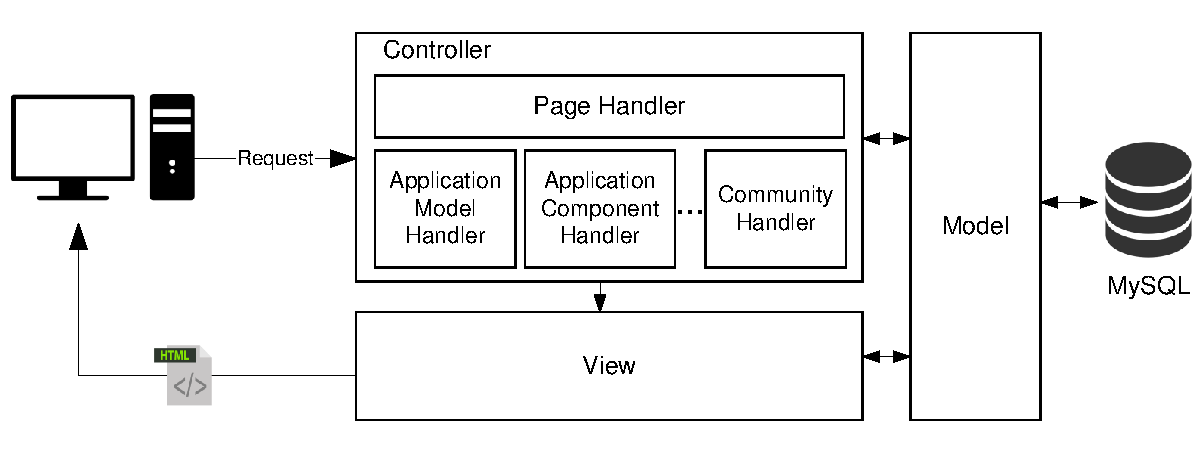
\includegraphics[width=0.6\textwidth,natwidth=200,natheight=150]{./fig/elgg_architecture.pdf}
	\centering
	\label{fig:elgg_architecture}
\end{figure}


All plugins share a common structure of folders and php files. Folder {\em actions} includes the actions applied on application models (delete, save, or search). The {\em views} folder contains the {\em php} forms applied on application models, {\em river} events (Elgg terminology for live feeds), and the application model editor. {\em Pages} overrides elements of core Elgg pages.  The {\em js} and {\em lib} folder provides javascript and {\em php} library functions. Finally, the {\em vendors} folders include third-party frameworks such as Twitter's bootstrap front-end.

Social network relationships (friendship, group, ownership, etc.) are persisted in the Elgg back-end database. The execution history of deployments of application models and the description of those models is stored in the CAMEL information repository, which is implemented as an Eclipse CDO server. The exchange of information between Elgg and the CDO server is implemented over sockets.

\section{Memcache}
\label{sec:memcache_implementation}
This section describes the experience gained by using memcached\cite{memcache_url}. Memcached is an open source, high-performance, distributed memory object caching system. We choose memcached, because is a generic simple in-memory key-value store. It has a powerful API available for PHP. After memcached integration the system increase the responce time and performance.

Memcached stores all entities of Social Network, applications, components, users, group discussions and most important the executions of applications. Storing the executions of applications at Memcached the responce time of the system increased because the PHP modules do not need to go through the heavy CDO client but get directly the executions of applications from Memcached.

The apache jmeter\cite{jmeter_url} was used to measure the responce time of the system and the sysstat tool\cite{sysstat_url} was used to measure the cpu usage.  

